\documentclass[tikz,border=12pt]{standalone}
% Shared visual language for standalone EMT block diagrams.
\usepackage{amsmath}
\usetikzlibrary{arrows.meta,backgrounds,calc,fit,positioning}

\tikzset{
    emt diagram/.style = {>={Stealth[length=2.4mm]}},
    line/.style        = {semithick, rounded corners=6pt},
    block/.style       = {draw, semithick, fill=white,
                          minimum height=1cm, minimum width=2.3cm},
    hblock/.style      = {block, minimum width=2.24cm, minimum height=1.3cm},
    vblock/.style      = {block, minimum width=1.3cm, minimum height=2.24cm},
    sum/.style         = {draw, semithick, fill=white, circle,
                          inner sep=2.6pt},
    signal/.style      = {circle, fill, inner sep=1.4pt,
                          label distance=3pt},
    sig/.style         = {font=\small},
    pm/.style          = {font=\scriptsize},
    wire jump/.style   = {line,
                          preaction={draw=white, line width=3pt,
                                     line cap=round}},
    enclosure/.style   = {draw, dashed, semithick, rounded corners=4pt},
    operator enclosure/.style = {enclosure, inner xsep=7mm, inner ysep=6mm}
}


% TUNABLES: channel spacing and gain-block width.
\def\channelspacing{2.8}
\def\gainwidth{1.25cm}

\begin{document}
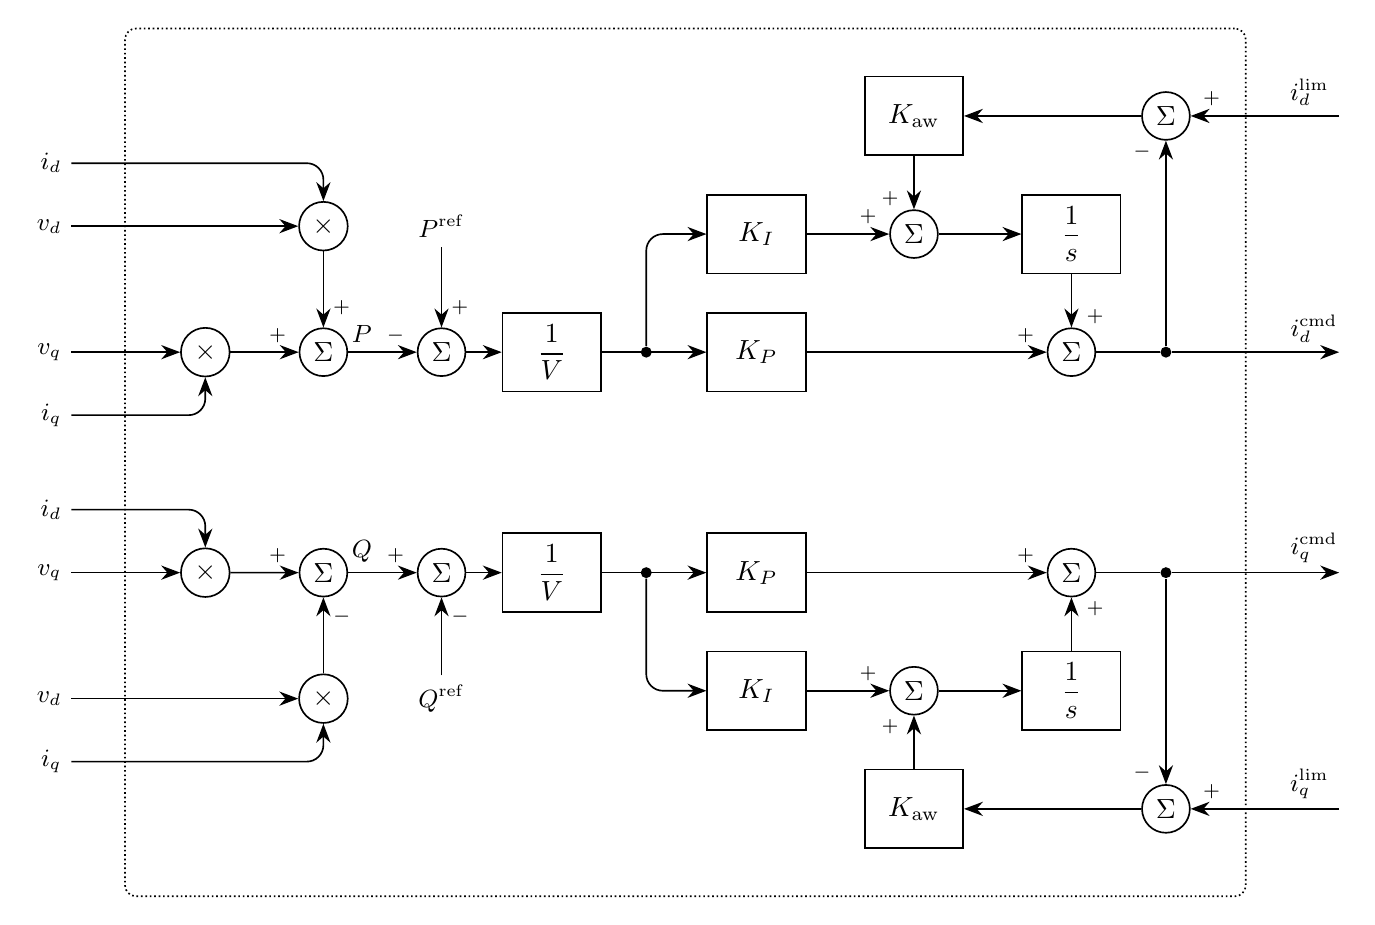
\begin{tikzpicture}[emt diagram]

% Local scalar measurements for each power product.
\foreach \name/\x/\y/\voltage/\current/\side/\dy in {
    pd/5.7/0.8/d/d/north/0.8,pq/4.2/-0.8/q/q/south/-0.8,
    qd/4.2/{-\channelspacing-0.8}/q/d/north/0.8,
    qq/5.7/{-\channelspacing-2.4}/d/q/south/-0.8} {
    \node[sum] (\name) at (\x,\y) {$\times$};
    \draw[->, line] (2.5,\y) node[sig, left] {$v_\voltage$}
        -- (\name.west);
    \draw[->, line] (2.5,\y+\dy) node[sig, left] {$i_\current$}
        -- (\x,\y+\dy) -- (\name.\side);
}

% Parallel d- and q-axis PI controllers with tracking anti-windup.
\foreach \axis/\offset/\power/\measured/\direction/\toward/\away in {
    d/0/P/-/-1/south/north,q/\channelspacing/Q/+/1/north/south} {
    \begin{scope}[yshift=-\offset cm]
        \node[sum] (power-\axis) at (5.7,-0.8) {$\Sigma$};
        \node[sum] (error-\axis) at (7.2,-0.8) {$\Sigma$};
        \node[block, minimum width=\gainwidth] (scale-\axis) at (8.6,-0.8) {$\dfrac{1}{V}$};
        \node[signal] (split-\axis) at (9.8,-0.8) {};
        \node[block, minimum width=\gainwidth] (Kp-\axis) at (11.2,-0.8) {$K_P$};
        \node[sum] (command-\axis) at (15.2,-0.8) {$\Sigma$};
        \node[signal] (output-\axis) at (16.4,-0.8) {};

        \draw[->, line] (power-\axis.east) -- node[sig, above, pos=0.2] {$\power$} (error-\axis.west);
        \node[pm, above left=0pt and 1pt of error-\axis.west] {$\measured$};
        \draw[->, line] (error-\axis.east) -- (scale-\axis.west);
        \draw[->, line] (scale-\axis.east) -- (Kp-\axis.west);
        \draw[->, line] (Kp-\axis.east) -- (command-\axis.west);
        \node[pm, above left=0pt and 1pt of command-\axis.west] {$+$};
        \draw[line] (command-\axis.east) -- (output-\axis);
        \draw[->, line] (output-\axis) -- node[sig, above, pos=0.85] {$i_\axis^{\mathrm{cmd}}$} (18.6,-0.8);

        \node[block, minimum width=\gainwidth] (Ki-\axis) at (11.2,{-0.8-1.5*\direction}) {$K_I$};
        \node[sum] (rate-\axis) at (13.2,{-0.8-1.5*\direction}) {$\Sigma$};
        \node[block, minimum width=\gainwidth] (integrator-\axis) at (15.2,{-0.8-1.5*\direction}) {$\dfrac{1}{s}$};
        \draw[->, line] (split-\axis) |- (Ki-\axis.west);
        \draw[->, line] (Ki-\axis.east) -- (rate-\axis.west);
        \node[pm, above left=0pt and 1pt of rate-\axis.west] {$+$};
        \draw[->, line] (rate-\axis.east) -- (integrator-\axis.west);
        \draw[->, line] (integrator-\axis.\toward) -- (command-\axis.\away);
        \node[pm, anchor=west] at ([xshift=2pt,yshift={-\direction*4pt}]command-\axis.\away) {$+$};

        \node[sum] (tracking-\axis) at (16.4,{-0.8-3*\direction}) {$\Sigma$};
        \node[block, minimum width=\gainwidth] (Kaw-\axis) at (13.2,{-0.8-3*\direction}) {$K_{\mathrm{aw}}$};
        \draw[->, line] (output-\axis) -- (tracking-\axis.\toward);
        \node[pm, anchor=east] at ([xshift=-2pt,yshift={\direction*4pt}]tracking-\axis.\toward) {$-$};
        \draw[->, line] (18.6,{-0.8-3*\direction}) -- node[sig, above, pos=0.2] {$i_\axis^{\mathrm{lim}}$} (tracking-\axis.east);
        \node[pm, above right=0pt and 1pt of tracking-\axis.east] {$+$};
        \draw[->, line] (tracking-\axis.west) -- (Kaw-\axis.east);
        \draw[->, line] (Kaw-\axis.\toward) -- (rate-\axis.\away);
        \node[pm, anchor=east] at ([xshift=-2pt,yshift={-\direction*4pt}]rate-\axis.\away) {$+$};
    \end{scope}
}

\draw[->, line] (pd.south) -- (power-d.north);
\node[pm, above right=1pt and 0pt of power-d.north] {$+$};
\draw[->, line] (pq.east) -- (power-d.west);
\node[pm, above left=0pt and 1pt of power-d.west] {$+$};
\draw[->, line] (qd.east) -- (power-q.west);
\node[pm, above left=0pt and 1pt of power-q.west] {$+$};
\draw[->, line] (qq.north) -- (power-q.south);
\node[pm, below right=1pt and 0pt of power-q.south] {$-$};

\node[sig] (pref) at (7.2,0.8) {$P^{\mathrm{ref}}$};
\draw[->, line] (pref.south) -- (error-d.north);
\node[pm, above right=1pt and 0pt of error-d.north] {$+$};
\node[sig] (qref) at (7.2,-\channelspacing-2.4) {$Q^{\mathrm{ref}}$};
\draw[->, line] (qref.north) -- (error-q.south);
\node[pm, below right=1pt and 0pt of error-q.south] {$-$};

\begin{scope}[on background layer]
    \node[operator enclosure, densely dotted,
        fit=(pd)(pq)(pref)(Kaw-d)(tracking-d)(Kp-d)(output-d)
            (qq)(Kaw-q)(tracking-q)] {};
\end{scope}

\end{tikzpicture}
\end{document}
